% Provenance (never printed): see sources/outline_sources.md (Year 3:
% energy-balance models, the one-layer model recalled; ice-albedo feedback
% and multiple equilibria; how general circulation models are built and
% evaluated).
% Brief: sources/book5/BRIEFS.md, ch. 22. Curves from
% figdata/bachelor-3/budyko_sellers.py (the zero-dimensional model and
% Budyko's latitudinal model; the brief's ebm_0d is folded into it) and
% two_layer.py. Exercise and problem values in the Book 5 scratch calculator
% calc/ch22.py. The model planet, model X and the ensemble of exercise 12 are
% invented.
\chapter{जलवायु मॉडल}\label{ch:b3:climate-models}

पृथ्वी तक पहुँचने वाले सूर्य के प्रकाश को लीजिए, जो पूरे गोले पर औसतन \qty{340}{W/m^2} है,
और उस अवरक्त विकिरण के लिए एक नियम लीजिए जिसे पृथ्वी अंतरिक्ष में लौटाती है,
जो प्रेक्षणों के तीस वर्षों के एक पुनर्विश्लेषण पर फ़िट किया गया है। मान लीजिए कि
जैसे-जैसे सतह ठंडी होती है, ग्रह का एल्बिडो खुली भूमि और समुद्र के एल्बिडो से
बढ़कर बर्फ़ के एल्बिडो तक पहुँच जाता है। दोनों फ़्लक्स को संतुलित कीजिए, तो
समीकरण के तीन हल होते हैं: \qty{14}{\celsius} पर एक ग्रह, जो वास्तविक पृथ्वी के
माध्य के निकट है; \qty{8}{\celsius} पर एक ग्रह; और \qty{-46}{\celsius} पर एक ग्रह,
जो ध्रुव से ध्रुव तक जमा हुआ है। जलवायु मॉडल, इन कुछ पंक्तियों से लेकर
सबसे बड़े कंप्यूटरों पर चलने वाले प्रोग्रामों तक, यह पूछने के उपकरण हैं कि किसी दिए गए
ग्रह की कौन-सी जलवायु है, वह वहाँ कैसे पहुँची, और उसके ऊर्जा-संतुलन में गड़बड़ी होने पर वह कैसे बदलती है।
% ledger: nasa:solar-mean, data:b5-ncep-air, data:b3-ncep, budyko69:albedo

\begin{recall}
कृष्णिका, स्टीफ़न--बोल्ट्ज़मान नियम, हरितगृह प्रभाव और
वायुमंडल का एक-परत मॉडल भौतिकी की पुस्तकों में हैं; एल्बिडो और
पृथ्वी का ऊर्जा बजट विद्यालय की पुस्तकों में। बाह्य दीर्घ-तरंग
विकिरण, उत्सर्जन तापमान और उत्तर-दक्षिण ऊष्मा परिवहन पुस्तक 3 (स्नातक वर्ष 1) में हैं,
उसके विकिरण और ऊष्मा परिवहन वाले अध्याय में। हिम--एल्बिडो प्रतिपुष्टि और
हिमगोल पृथ्वी पुस्तक 4 (स्नातक वर्ष 2) में हैं, उसके
प्रीकैम्ब्रियन पृथ्वी वाले अध्याय में; प्रभावी विकिरणी,
जलवायु प्रतिपुष्टि प्राचल $\lambda < 0$, साम्य जलवायु संवेदनशीलता
(ECS) और क्षणिक जलवायु अनुक्रिया (TCR) उसके
मानवजनित जलवायु परिवर्तन वाले अध्याय में; संख्यात्मक मौसम पूर्वानुमान और
समष्टि पूर्वानुमान उसके मौसम तंत्र वाले अध्याय में। घूमती पृथ्वी पर गति के
समीकरण, \omterm{def:b3:gfd-foundations:hydrostatic}{द्रवस्थैतिक सन्निकटन} के साथ,
अध्याय~\ref{ch:b3:gfd-foundations} में हैं।
\end{recall}

\section{ग्रह का ऊर्जा-संतुलन}\label{sec:b3:climate-models:zero-d}

गोले पर और एक वर्ष पर औसत लेने पर, वायुमंडल के शीर्ष पर हर वर्ग मीटर को
$Q = S_0/4 = \qty{340}{W/m^2}$ प्राप्त होता है, जो
सौर विकिरण-तीव्रता $S_0 = \qty{1360}{W/m^2}$ का एक-चौथाई है। एक भाग $\alpha$, जिसे
ग्रह का एल्बिडो कहते हैं, परावर्तित हो जाता है; शेष $Q(1 - \alpha)$ अवशोषित होता है
और अवरक्त के रूप में अंतरिक्ष में लौटाया जाना चाहिए। एक कृष्णिका $\sigma
T^4$ उत्सर्जित करती; पृथ्वी का बाह्य दीर्घ-तरंग विकिरण (OLR) इससे कम है,
हरितगृह प्रभाव के कारण, और पृथ्वी पर पाए जाने वाले सतह-तापमानों की परास में
वह लगभग एक सीधी रेखा है,
\[
\text{OLR} = A + BT ,
\]
जहाँ $T$ डिग्री सेल्सियस में सतह का तापमान है। 1969 में बुडिको ने
260 केंद्रों पर परिकलित बाह्य विकिरण पर ऐसा ही एक नियम फ़िट किया, मेघाच्छादन
$n$ के लिए एक सुधार के साथ: $I = a + bT - (a_1 + b_1T)n$, $a = 14.0$, $b = 0.14$, $a_1 =
3.0$ और $b_1 = 0.10$ के साथ, \unit{kcal.cm^{-2}} प्रति माह में, और
\qty{5}{\percent} से कम प्रकीर्णन के साथ। मेघाच्छादन के माध्य 0.5 के लिए यह $A =
\qty{199}{W/m^2}$ और $B = \qty{1.43}{W.m^{-2}.\celsius^{-1}}$ देता है। वार्षिक
\omterm{def:b3:atmospheric-dynamics:eddy}{आंचलिक माध्य}, NCEP--NCAR पुनर्विश्लेषण~1 के 1991--2020 के लिए, क्षेत्रफल से भारित,
$A = \qty{211.9}{W/m^2}$ और $B = \qty{1.816}{W.m^{-2}.\celsius^{-1}}$ देते हैं,
रेखा के चारों ओर \qty{10}{W/m^2} के प्रकीर्णन के साथ। नीचे ये मान
प्रयोग किए जाते हैं।
% ledger: nasa:solar-mean, budyko69:olr, data:b5-ncep-air, data:b3-ncep

\begin{definition}[ऊर्जा-संतुलन मॉडल]\label{def:b3:climate-models:ebm}
एक \emph{ऊर्जा-संतुलन मॉडल}\index{ऊर्जा-संतुलन मॉडल} एक जलवायु मॉडल है जो सतह
का तापमान परिकलित करता है --- एक एकल वैश्विक माध्य, या हर अक्षांश पर एक माध्य ---
अवशोषित सूर्य के प्रकाश, अंतरिक्ष में उत्सर्जित अवरक्त
और, यदि तापमान अक्षांश पर निर्भर है, तो
ध्रुवों की ओर ले जाई गई ऊष्मा के संतुलन से। इसके शून्य-आयामी रूप में
\[
C\,\frac{\mathrm dT}{\mathrm dt} = Q\big(1 - \alpha(T)\big) - (A + BT) ,
\]
जहाँ $C$ तंत्र के उस भाग की प्रति एकक क्षेत्रफल ऊष्माधारिता है जो
सतह के साथ गर्म होता है।
\end{definition}

$\alpha = 0.30$ के साथ साम्य है $T = (238 - 211.9)/1.816 =
\qty{14.4}{\celsius}$; पुनर्विश्लेषण का क्षेत्रीय माध्य
\qty{14.2}{\celsius} है। कार्बन डाइऑक्साइड के परिवर्तन जैसा एक बल $F$
दाईं ओर जुड़ता है। किसी साम्य के निकट अनुक्रिया
पुस्तक 4 (स्नातक वर्ष 2) के जलवायु प्रतिपुष्टि प्राचल $\lambda$ से नियंत्रित होती है:
एल्बिडो स्थिर होने पर, $\lambda = -B$।
% ledger: earth:albedo, data:b5-ncep-air

\begin{theorem}[एक-बक्सा जलवायु की अनुक्रिया-काल]\label{thm:b3:climate-models:response}
मान लीजिए कोई जलवायु साम्य में है, और एक स्थिर बल $F$
$t = 0$ पर चालू किया जाता है। यदि साम्य से विचलन $T'$ $C\,\mathrm
dT'/\mathrm dt = F + \lambda T'$ का पालन करता है, जहाँ $C > 0$ और $\lambda < 0$ स्थिर हैं,
तो
\[
T'(t) = -\frac{F}{\lambda}\Big(1 - \mathrm e^{-t/\tau}\Big), \qquad
\tau = -\frac{C}{\lambda} .
\]
नया साम्य $-F/\lambda$ है, और जलवायु $1
- \mathrm e^{-1} = \num{0.63}$ भाग का मार्ग समय $\tau$ में तय कर लेती है।
\end{theorem}

\begin{proof}
$T'_\infty = -F/\lambda$ दाईं ओर को शून्य कर देता है। अंतर
$u = T' - T'_\infty$ का पालन करता है $C\,\mathrm du/\mathrm dt = \lambda u$, इसलिए $u =
u(0)\,\mathrm e^{\lambda t/C}$, जहाँ $u(0) = F/\lambda$।
\end{proof}

कुछ वर्षों में जो ऊष्माधारिता मायने रखती है, वह ऊपरी महासागर की है।
जलवायु परिवर्तन पर अंतर-सरकारी पैनल की छठी आकलन रिपोर्ट का द्वि-परत एमुलेटर,
जो 44 जलवायु मॉडलों पर अंशांकित है,
सतह परत के लिए $C = \qty{8.1}{W.yr.m^{-2}.\celsius^{-1}}$ मान देता है,
जो \qty{62}{m} गहरे समुद्री जल की एक परत की ऊष्माधारिता है। $\lambda = -B$ के साथ
अनुक्रिया-काल $8.1/1.816 = \num{4.5}\text{ वर्ष}$ है। वास्तविक जलवायु
गहन महासागर को भी गर्म करती है, बहुत धीरे; अनुभाग~\ref{sec:b3:climate-models:two-layer}
इसे जोड़ता है।
% ledger: ar6sm7:two-layer, teos10:cp0, data:b5-ncep-air

\section{हिम, एल्बिडो और बहु साम्यावस्थाएँ}\label{sec:b3:climate-models:multiple}

पुस्तक 4 (स्नातक वर्ष 2) की हिम--एल्बिडो प्रतिपुष्टि एल्बिडो को
तापमान पर निर्भर बनाती है। मान लीजिए ऐसे ग्रह के लिए $\alpha = 0.62$ है, जिसकी सतह
$T_I = \qty{-10}{\celsius}$ से नीचे है, बुडिको के मॉडल में बर्फ़ का एल्बिडो, $\alpha
= 0.30$ है और $T_F = \qty{+10}{\celsius}$ से ऊपर, इनके बीच एक सीधी रेखा, जैसे-जैसे बर्फ़ पीछे हटती है।
रैंप इस अध्याय का एक चुनाव है; कोई भी एल्बिडो जो
ग्रह ठंडा होने पर बढ़ता है, वही तस्वीर देता है।
% ledger: budyko69:albedo, earth:albedo

\begin{definition}[बहु जलवायु साम्यावस्थाएँ; सैडल-नोड द्विभाजन]\label{def:b3:climate-models:multiple-equilibria}
किसी जलवायु मॉडल में \emph{बहु जलवायु साम्यावस्थाएँ}\index{बहु जलवायु साम्यावस्थाएँ} तब होती हैं
जब समान बाह्य परिस्थितियों के लिए उसकी एक से अधिक
स्थायी अवस्थाएँ हों। कोई साम्यावस्था स्थिर होती है यदि उससे छोटा विचलन क्षय हो जाए,
और अस्थिर यदि वह बढ़े। एक \emph{सैडल-नोड
द्विभाजन}\index{सैडल-नोड द्विभाजन} वह प्राचल का मान है जिस पर एक स्थिर और एक अस्थिर साम्यावस्था
आपस में मिलती हैं और एक साथ लुप्त हो जाती हैं।
\end{definition}

\begin{proposition}[तीन साम्यावस्थाएँ और उनकी स्थिरता]\label{prop:b3:climate-models:three}
मान लीजिए शुद्ध अधोमुखी फ़्लक्स $N(T) = Q(1 - \alpha(T)) - (A + BT)$ है। एक
साम्यावस्था $T^*$, $N(T^*) = 0$, स्थिर है यदि $N'(T^*) < 0$ और
अस्थिर है यदि $N'(T^*) > 0$। ऊपर के रैंप के साथ $N' = -B$ हिमगोल और बर्फ़-मुक्त शाखाओं पर है,
जो जहाँ भी विद्यमान हैं, वहाँ स्थिर हैं, और $N' = -B -
Q\,\mathrm d\alpha/\mathrm dT$ रैंप पर, जो तब अस्थिर है जब $Q\,
|\mathrm d\alpha/\mathrm dT| > B$। $Q = \qty{340}{W/m^2}$ के लिए मॉडल में
तीन साम्यावस्थाएँ हैं, \qty{-45.5}{\celsius} (स्थिर), \qty{7.8}{\celsius}
(अस्थिर) और \qty{14.4}{\celsius} (स्थिर)।
\end{proposition}

\begin{proof}
$T^*$ के निकट $C\,\mathrm dT'/\mathrm dt = N'(T^*)T'$ है, जो क्षय करता है यदि
$N'(T^*) < 0$ और बढ़ता है यदि $N'(T^*) > 0$। रैंप पर $\mathrm d\alpha/
\mathrm dT = -0.32/20 = \qty{-0.016}{\celsius^{-1}}$ है, अतः $N' = -1.816 + 340
\times 0.016 = \qty{+3.62}{W.m^{-2}.\celsius^{-1}}$। हिमगोल शाखा,
$T = (340\times0.38 - 211.9)/1.816 = \qty{-45.5}{\celsius}$ पर, $T_I$ से नीचे स्थित है;
गरम वाली \qty{14.4}{\celsius} पर, $T_F$ से ऊपर; रैंप पर
$340(0.54 + 0.016\,T) = 211.9 + 1.816\,T$ से $T = \qty{7.8}{\celsius}$ प्राप्त होता है।
\end{proof}

\begin{omfigure}
\begin{tikzpicture}
\begin{groupplot}[group style={group size=2 by 1, horizontal sep=1.5cm},
  width=0.48\linewidth, height=0.4\linewidth,
  tick label style={font=\scriptsize}, label style={font=\small}, title style={font=\small}]
\nextgroupplot[xlabel={$T$ (\unit{\celsius})}, ylabel={फ़्लक्स (\unit{W/m^2})},
  xmin=-60, xmax=40, ymin=80, ymax=270, title={$Q = \qty{340}{W/m^2}$ पर संतुलन},
  legend style={font=\scriptsize, at={(0.03,0.97)}, anchor=north west}]
% computed in figdata/bachelor-3/budyko_sellers.py
\addplot[omThm, thick] table[x=T, y=asr] {figdata/out/bachelor-3-budyko_sellers-asr.dat};
\addlegendentry{अवशोषित सूर्यप्रकाश}
\addplot[omDef, thick] table[x=T, y=olr] {figdata/out/bachelor-3-budyko_sellers-olr.dat};
\addlegendentry{$A + BT$}
\addplot[only marks, mark=*, mark size=2pt, forget plot] coordinates {(-45.55,129.2) (14.38,238.0)};
\addplot[only marks, mark=o, mark size=2pt, thick, forget plot] coordinates {(7.81,226.07)};
\node[font=\scriptsize, anchor=north west] at (axis cs:-45.55,125) {हिमगोल};
\draw[black!60] (axis cs:7.81,226.07) -- (axis cs:16,200);
\node[font=\scriptsize, anchor=north west, inner sep=1pt] at (axis cs:16,200) {अस्थिर};
\nextgroupplot[xlabel={$S_0$ (\unit{W/m^2})}, ylabel={$T$ (\unit{\celsius})},
  xmin=1000, xmax=2200, ymin=-70, ymax=100, title={साम्यावस्थाएँ और हिस्टैरिसिस},
  scaled x ticks=false, xticklabel style={/pgf/number format/1000 sep={}}]
\addplot[black!40, densely dotted, forget plot] coordinates {(1360,-70) (1360,100)};
\addplot[omMeth, thick] table[x=S, y=T] {figdata/out/bachelor-3-budyko_sellers-eqwarm.dat};
\addplot[omThm, thick] table[x=S, y=T] {figdata/out/bachelor-3-budyko_sellers-eqcold.dat};
\addplot[black!60, thick, dashed] table[x=S, y=T] {figdata/out/bachelor-3-budyko_sellers-eqmid.dat};
\draw[->, thick, black!70] (axis cs:1314.6,8) -- (axis cs:1314.6,-45);
\draw[->, thick, black!70] (axis cs:2039.4,-8) -- (axis cs:2039.4,77);
\node[font=\scriptsize, anchor=south, black!60, fill=white, inner sep=1pt] at (axis cs:1360,84) {आज};
\node[font=\scriptsize, omMeth, anchor=north west] at (axis cs:1700,32) {गरम};
\node[font=\scriptsize, omThm, anchor=north] at (axis cs:1620,-40) {हिमगोल};
\end{groupplot}
\end{tikzpicture}

\par\smallskip{\small शून्य-आयामी \omterm{def:b3:climate-models:ebm}{ऊर्जा-संतुलन मॉडल}, जिसमें एक
हिम--एल्बिडो रैंप है और OLR नियम NCEP--NCAR पुनर्विश्लेषण~1 पर फ़िट किया गया है।
बाएँ, आज के सूर्यप्रकाश के लिए अवशोषित सूर्यप्रकाश और उत्सर्जित अवरक्त:
ये तीन बार एक-दूसरे को काटते हैं; भरे वृत्त स्थिर हैं, खुला वृत्त अस्थिर।
दाएँ, साम्य तापमान बनाम सौर स्थिरांक, स्थिर
शाखाएँ ठोस, अस्थिर वाली बिंदीदार। आज के मान से सूर्य को घटाने पर
गरम ग्रह ठंडा होता है, जब तक गरम शाखा
\qty{1315}{W/m^2} पर समाप्त होती है, और जलवायु हिमगोल की ओर गिर जाती है; वह जमी रहती है
जब तक सूर्य को \qty{2039}{W/m^2} तक नहीं उठाया जाता, जहाँ वह
एकाएक एक अत्यंत गरम ग्रह पर लौट आती है, उस परास से कहीं आगे
जिसमें सीधी-रेखा वाला OLR नियम मान्य है।}\label{fig:b3:climate-models:zero-d}
\end{omfigure}
% ledger: nasa:solar-mean, data:b5-ncep-air, budyko69:albedo, earth:albedo

जैसे-जैसे $Q$ घटता है, गरम साम्यावस्था ठंडी होती है और रैंप वाली साम्यावस्था गरम होती है।
ये रैंप के शिखर पर मिलती हैं, $T = T_F$ पर, जहाँ $Q(1 - 0.30) = A +
10B$: $Q = \qty{328.7}{W/m^2}$, जो \qty{1315}{W/m^2} का सौर स्थिरांक है,
आज के मान से \qty{3.3}{\percent} कम। यह एक \omterm{def:b3:climate-models:multiple-equilibria}{सैडल-नोड द्विभाजन} है: इससे नीचे
एकमात्र साम्यावस्था हिमगोल है, और जलवायु उसी में गिर जाती है।
सूर्य को फिर उठाने से गरम ग्रह वापस नहीं आता: हिमगोल
शाखा तभी समाप्त होती है जब उसका तापमान $T_I$ तक पहुँचता है, $Q(1 - 0.62) = A -
10B$, सौर स्थिरांक \qty{2039}{W/m^2} पर, आज के
मान से \qty{50}{\percent} ऊपर। इन दोनों के बीच ग्रह की अवस्था उसके इतिहास पर निर्भर करती है:
मॉडल में हिस्टैरिसिस है। वास्तविक नियोप्रोटेरोज़ोइक में
पुस्तक 4 (स्नातक वर्ष 2) वाले हिमगोल से निकलने का रास्ता चमकीला सूर्य नहीं, बल्कि ज्वालामुखियों की
कार्बन डाइऑक्साइड थी, जो लाखों वर्षों में जमा होती रही, जब तक ग्रीनहाउस
प्रणोदन हिमविगलन की सीमा तक पहुँचा; तब हिम-रेखा ध्रुवों की ओर
कुछ हज़ार वर्षों में पीछे हट गई।
% ledger: hoffman17:hysteresis

\section{बुडिको--सेलर्स मॉडल}\label{sec:b3:climate-models:budyko-sellers}

एक ही तापमान से हिम-रेखा नहीं बनती। 1969 में बुडिको ने तापमान को
अक्षांश पर निर्भर रखा और पूछा कि सूर्यप्रकाश में कमी
हिम को भूमध्य रेखा की ओर कितनी दूर धकेलेगी।

\begin{definition}[बुडिको--सेलर्स मॉडल]\label{def:b3:climate-models:budyko-sellers}
\emph{बुडिको--सेलर्स मॉडल}\index{बुडिको--सेलर्स मॉडल} एक
\omterm{def:b3:climate-models:ebm}{ऊर्जा-संतुलन मॉडल} है, जिसमें वार्षिक माध्य तापमान $T(x)$
$x = \sin\varphi$ पर निर्भर करता है, जहाँ $\varphi$ अक्षांश है, और गोलार्ध सममित हैं।
प्रत्येक अक्षांश पर
\[
C\,\frac{\partial T}{\partial t} = Qs(x)\big(1 - \alpha(x)\big) - (A + BT) - D(x) ,
\]
जहाँ $s(x)$ उस अक्षांश के वार्षिक सूर्यातप का अपने वैश्विक
माध्य से भाग है, $D(x)$ ध्रुवाभिमुख ऊष्मा परिवहन का अपसरण है, और एल्बिडो
ध्रुवों की ओर हिम-रेखा $x_s$ के पार अपना हिम-मान लेता है, जहाँ $T$ एक
क्रांतिक तापमान $T_c$ से नीचे गिरता है। बुडिको ने $D = \beta(T - \bar T)$ लिखा, जो
वैश्विक माध्य $\bar T$ की ओर शिथिलन है; विसरणी रूप में, $D =
-\mathcal D\,\partial_x\big[(1 - x^2)\,\partial_xT\big]$.
\end{definition}

गुणक $x = \sin\varphi$ इसलिए चुना जाता है, क्योंकि $x$ के समान अंतराल
गोले के समान क्षेत्रफल घेरते हैं, ताकि वैश्विक माध्य $\int_0^1\cdot\,\mathrm
dx$ होता है। बुडिको ने $\beta = \qty{0.235}{kcal.cm^{-2}}$ प्रति माह और प्रति अंश पाया,
\qty{3.74}{W.m^{-2}.\celsius^{-1}}, जो अक्षांश के साथ तापमान के प्रेक्षित
वितरण से निकला। उन्होंने हिम पर एल्बिडो 0.62 और उसके किनारे पर 0.50 रखा,
जहाँ हिम टूटी हुई है, और वर्तमान हिम-किनारे को औसत
अक्षांश \ang{72} N पर लिया; क्रांतिक तापमान वह है जो किनारे को
ठीक वहीं रखता है।
% ledger: budyko69:transport, budyko69:albedo

\begin{proposition}[बुडिको के मॉडल की हिम-रेखा]\label{prop:b3:climate-models:iceline}
मान लीजिए $F(x_s) = \int_0^{x_s}s\,\mathrm dx$ सूर्यप्रकाश का वह भाग है जो
हिम-रेखा के भूमध्य की ओर पड़ता है, और $\bar\alpha = \alpha_FF + \alpha_I(1 -
F)$ सूर्यप्रकाश से भारित माध्य एल्बिडो है। बुडिको के
मॉडल की स्थायी अवस्था में,
\[
B\bar T = Q(1 - \bar\alpha) - A, \qquad
T(x) = \frac{Qs(x)\big(1 - \alpha(x)\big) - A + \beta\bar T}{B + \beta} ,
\]
और $x_s$ पर हिम-रेखा, जहाँ $T = T_c$ और किनारे का एल्बिडो $\alpha_e$ है,
उसके लिए निम्न संबंध आवश्यक है:
\[
Q(x_s) = \frac{(B + \beta)T_c + A(1 + \beta/B)}{s(x_s)(1 - \alpha_e) +
(\beta/B)\big(1 - \bar\alpha(x_s)\big)} .
\]
हिम-रेखा वहाँ स्थायी है जहाँ $\mathrm dQ/\mathrm dx_s > 0$ है, और
वहाँ अस्थायी है जहाँ $\mathrm dQ/\mathrm dx_s < 0$ है।
\end{proposition}

\begin{proof}
स्थायी संतुलन को $0 \le x \le 1$ पर समाकलित करने पर परिवहन पद
लुप्त हो जाता है, क्योंकि $\int_0^1(T - \bar T)\,\mathrm dx = 0$ है, और $\int_0^1
s(1 - \alpha)\,\mathrm dx = 1 - \bar\alpha$ है; इससे $\bar T$ प्राप्त होता है। प्रत्येक
$x$ पर स्थायी संतुलन $T(x)$ में रैखिक होता है। $T(x_s) = T_c$ रखकर
और $\bar T$ को उसके मान से बदलने पर अंतिम सूत्र प्राप्त होता है, जो $Q$ में रैखिक है।
स्थायित्व का प्रतिबंध स्वीकार किया गया है: यह स्थायी अवस्था के चारों ओर
समय-आश्रित मॉडल के रैखिकीकरण से निकलता है।
\end{proof}

इसका अर्थ शून्य-आयामी मॉडल वाला ही है: स्थायी शाखा के साथ
थोड़ा अधिक सूर्यप्रकाश हिम-रेखा को ध्रुव की ओर धकेलता है। वह तापमान
जिस पर किनारा आज स्थित है, $T_c = \qty{-12.3}{\celsius}$ तय करता है; पुनर्विश्लेषण
\ang{72} पर \qty{-15.8}{\celsius} देता है, जो दोनों
गोलार्धों का माध्य है। मॉडल की नीचे दी गई रूपरेखा उष्णकटिबंध में
प्रेक्षित रूपरेखा से ठंडी है, और ध्रुवों के निकट कहीं अधिक गर्म: एक अकेला गुणांक $\beta$
पूरी रूपरेखा में फिट नहीं बैठ सकता। इसका वैश्विक माध्य,
\qty{12.8}{\celsius} और भूमध्य रेखा पर इसका तापमान, \qty{22.8}{\celsius},
प्रेक्षित \qty{14.2}{\celsius} और \qty{25.7}{\celsius} के निकट हैं।
% ledger: data:b5-ncep-air, data:b3-ncep, budyko69:albedo

\begin{omfigure}
\begin{tikzpicture}
\begin{groupplot}[group style={group size=2 by 1, horizontal sep=1.5cm},
  width=0.48\linewidth, height=0.42\linewidth,
  tick label style={font=\scriptsize}, label style={font=\small}, title style={font=\small}]
\nextgroupplot[xlabel={$Q/Q_0$}, ylabel={हिम-रेखा अक्षांश (\unit{\degree})},
  xmin=0.95, xmax=1.25, ymin=-3, ymax=93, ytick={0,15,30,45,60,75,90},
  title={सूर्यप्रकाश के सापेक्ष हिम-रेखा}, clip=false,
  scaled x ticks=false, xticklabel style={/pgf/number format/fixed, /pgf/number format/precision=2}]
% computed in figdata/bachelor-3/budyko_sellers.py
\addplot[black!40, densely dotted] coordinates {(1,-3) (1,93)};
\addplot[omMeth, thick] table[x=q, y=lat] {figdata/out/bachelor-3-budyko_sellers-icestable.dat};
\addplot[black!60, thick, dashed] table[x=q, y=lat] {figdata/out/bachelor-3-budyko_sellers-iceunstable.dat};
\addplot[omThm, thick] coordinates {(0.95,0) (1.2249,0)};
\addplot[omMeth, thick] coordinates {(1.0069,90) (1.25,90)};
\addplot[only marks, mark=*, mark size=2pt] coordinates {(1,72) (1,0) (0.9713,47.65)};
\addplot[only marks, mark=o, mark size=2pt, thick] coordinates {(1,30.15)};
\node[font=\scriptsize, anchor=west] at (axis cs:1.005,72) {आज};
\draw[black!60] (axis cs:0.9713,47.65) -- (axis cs:1.02,50);
\node[font=\scriptsize, anchor=west, align=left] at (axis cs:1.02,50) {हिमनद सीमा};
\node[font=\scriptsize, omThm, anchor=south] at (axis cs:1.06,1) {हिमगोल};
\node[font=\scriptsize, omMeth, anchor=north] at (axis cs:1.15,89) {बिना हिम};
\nextgroupplot[xlabel={अक्षांश (\unit{\degree})}, ylabel={$T$ (\unit{\celsius})},
  xmin=0, xmax=90, xtick={0,15,30,45,60,75,90}, ymin=-35, ymax=32, title={आज का तापमान},
  legend style={font=\scriptsize, at={(0.03,0.03)}, anchor=south west}]
\addplot[omDef, thick] table[x=lat, y=tmodel] {figdata/out/bachelor-3-budyko_sellers-profile.dat};
\addlegendentry{बुडिको मॉडल}
\addplot[black, thick, mark=*, mark size=0.9pt] table[x=lat, y=tobs] {figdata/out/bachelor-3-budyko_sellers-obs.dat};
\addlegendentry{पुनर्विश्लेषण}
\addplot[black!50, densely dashed] coordinates {(0,-12.26) (90,-12.26)};
\addlegendentry{$T_c$}
\end{groupplot}
\end{tikzpicture}

\par\smallskip{\small बुडिको का अक्षांशीय मॉडल, पुनर्विश्लेषण के OLR नियम और
प्रत्येक अक्षांश के सूर्यातप के साथ। बाईं ओर, $Q/Q_0$ वह सूर्यप्रकाश है जो
हिम-रेखा को प्रत्येक अक्षांश पर बनाए रखने के लिए चाहिए: स्थायी शाखा ठोस, अस्थायी
रेखांकित। आज $Q/Q_0 = 1$ है, तीन अवस्थाएँ साथ रहती हैं: हिम-रेखा \ang{72} पर
(स्थायी), \ang{30} पर (अस्थायी) और हिमगोल। स्थायी शाखा समाप्त होती है
अपने न्यूनतम पर, \ang{47.7} और \num{0.9713} पर: वहाँ कम सूर्यप्रकाश से
बर्फ़ भूमध्य रेखा तक चली जाती है। दाईं ओर, मॉडल का आज का तापमान
1991--2020 के NCEP--NCAR पुनर्विश्लेषण~1 के वार्षिक \omterm{def:b3:atmospheric-dynamics:eddy}{आंचलिक माध्य} के विरुद्ध, दोनों गोलार्धों पर औसत लिया गया;
हिम-रेखा वहाँ है जहाँ किनारे के एल्बिडो के साथ मॉडल का वक्र
$T_c$ तक पहुँचता है।}\label{fig:b3:climate-models:budyko}
\end{omfigure}
% ledger: data:b5-ncep-air, data:b3-ncep, budyko69:albedo, budyko69:transport

स्थायी शाखा का एक न्यूनतम है। इन मानों के साथ वह \ang{47.7} पर है,
$Q/Q_0 = \num{0.9713}$ के लिए: सूर्यप्रकाश में \qty{2.87}{\percent} की कमी
हिम को मध्य अक्षांशों तक ले आती है, और इससे आगे की कोई भी कमी उसे
भूमध्य रेखा तक भेज देती है। बुडिको ने अपने स्वयं के गुणांकों के साथ एक छोटी सीमा पाई:
\qty{1.6}{\percent} की कमी ने उनकी हिम को लगभग
\ang{50} के औसत अक्षांश तक पहुँचाया, जिसके बाद वह स्वतः भूमध्य रेखा की ओर बढ़ गई और
औसत तापमान शून्य से कई दर्जन अंश नीचे गिर गया। OLR और एल्बिडो का फिट
संख्या को बदलता है; वक्र की आकृति, उसका न्यूनतम और
उसके आगे का अनियंत्रित विस्तार नहीं बदलते। मॉडल का विसरणी रूप, जिसे
$x$ में लीजेंडर बहुपदों से हल किया जाता है, वही आकृति देता है (अभ्यास~\ref{exo:b3:climate-models:10}
बिना हिम वाले ग्रह से निपटता है)।
% ledger: budyko69:threshold, hoffman17:hysteresis

\section{द्वि-परत मॉडल}\label{sec:b3:climate-models:two-layer}

एक-बॉक्स मॉडल का प्रतिक्रिया काल, जो कुछ वर्ष है, ऊपरी
महासागर का है। उसके नीचे गहन महासागर सदियों तक ऊष्मा अवशोषित करता है,
और जब तक वह ऐसा करता है, सतह अपने साम्य से ठंडी रहती है।

\begin{definition}[द्वि-परत ऊर्जा-संतुलन मॉडल]\label{def:b3:climate-models:two-layer}
\emph{द्वि-परत ऊर्जा-संतुलन मॉडल}\index{द्वि-परत ऊर्जा-संतुलन मॉडल} जलवायु को
एक सतही परत से, जिसका तापमान विचलन $T$
और ऊष्मा धारिता $C$ है, तथा एक गहन महासागर से, जिसका तापमान विचलन $T_d$ और
ऊष्मा धारिता $C_d$ है, ऊष्मा-विनिमय गुणांक $\gamma > 0$ से युग्मित करके निरूपित करता है:
\[
C\,\frac{\mathrm dT}{\mathrm dt} = F + \lambda T - \gamma(T - T_d), \qquad
C_d\,\frac{\mathrm dT_d}{\mathrm dt} = \gamma(T - T_d) .
\]
\end{definition}

\begin{theorem}[तीव्र और मंद अनुक्रियाएँ]\label{thm:b3:climate-models:two-layer}
माना $\lambda < 0$, $\gamma > 0$, $C, C_d > 0$ है, और एक स्थिर बल
$F$, जो $t = 0$ पर साम्य से आरंभ होता है, तब
\[
T(t) = -\frac{F}{\lambda}\Big(1 - a_f\,\mathrm e^{-t/\tau_f} - a_s\,\mathrm
e^{-t/\tau_s}\Big), \qquad a_f + a_s = 1 ,
\]
जहाँ $1/\tau_f$ और $1/\tau_s$ निम्न द्विघात समीकरण के मूल हैं: $r^2 - \big((\gamma -
\lambda)/C + \gamma/C_d\big)r - \lambda\gamma/(CC_d) = 0$। जब $C \ll C_d$ हो,
\[
\tau_f \approx \frac{C}{\gamma - \lambda}, \qquad
\tau_s \approx \frac{C_d(\gamma - \lambda)}{-\lambda\gamma}, \qquad
a_f \approx \frac{-\lambda}{\gamma - \lambda} .
\]
\end{theorem}

\begin{proof}
साम्य $T = T_d = -F/\lambda$ है। इससे विचलन
$\mathrm d\vec u/\mathrm dt = M\vec u$ के अनुसार चलते हैं, जहाँ
\[
M = \begin{pmatrix} (\lambda - \gamma)/C & \gamma/C\\ \gamma/C_d &
-\gamma/C_d\end{pmatrix}, \qquad
\operatorname{tr}M = -\frac{\gamma - \lambda}{C} - \frac{\gamma}{C_d},
\qquad \det M = \frac{-\lambda\gamma}{CC_d} > 0 ,
\]
अतः दोनों आइगेनमान $-r$ वास्तविक और ऋणात्मक हैं, और $r$ उस द्विघात समीकरण को संतुष्ट करता है
जो कथन में है। $\vec u$ का प्रत्येक घटक दो घातांकीय पदों का संयोजन होता है: $\mathrm
e^{-t/\tau_f}$ और $\mathrm e^{-t/\tau_s}$; $T(0) = 0$ से $a_f + a_s =
1$ प्राप्त होता है। यदि $C \ll C_d$ हो, तो बड़ा मूल ट्रेस के निकट होता है, $(\gamma -
\lambda)/C$ के निकट, और छोटा मूल सारणिक को उसी से भाग देने पर मिलता है। तीव्र
समय-पैमाने पर गहन महासागर अभी तक नहीं बदला है, $T_d \approx 0$, और सतह
$F/(\gamma - \lambda)$ पर स्थिर होती है, जो अंतिम तापन का
भाग $-\lambda/(\gamma - \lambda)$ है, यानी $a_f$।
\end{proof}

मूल्यांकन के एमुलेटर में, जो 44 मॉडलों पर अंशांकित है, $C =
\qty{8.1}{W.yr.m^{-2}.\celsius^{-1}}$, $C_d = \qty{110}{W.yr.m^{-2}.\celsius^{-1}}$
और $\gamma = \qty{0.62}{W.m^{-2}.\celsius^{-1}}$ है; इसका प्रतिपुष्टि प्राचल
लगभग $\lambda = \qty{-1.33}{W.m^{-2}.\celsius^{-1}}$ पर नमूना लिया गया है। ये मान
$\tau_f = \num{4.1}\text{ वर्ष}$ और $\tau_s = \num{262}\text{ वर्ष}$ देते हैं, साथ ही $a_f =
0.67$: \qty{62}{\percent} तापन एक दशक के भीतर आ जाता है, शेष अधिकांश
सदियों में आता है। एमुलेटर पहले समीकरण के ऊष्मा-विनिमय को भी
प्रभाविता $\varepsilon = 1.34$ से गुणा करता है, जो सतह को
और धीमा कर देता है; यहाँ इसे 1 रखा गया है।
% ledger: ar6sm7:two-layer

\begin{omfigure}
\begin{tikzpicture}
\begin{groupplot}[group style={group size=2 by 1, horizontal sep=1.4cm},
  width=0.48\linewidth, height=0.4\linewidth,
  tick label style={font=\scriptsize}, label style={font=\small}, title style={font=\small},
  ylabel={तापन (\unit{\celsius})}]
\nextgroupplot[xlabel={चरण के बाद वर्ष}, xmin=0, xmax=500, ymin=0, ymax=6.6,
  title={अचानक चौगुना},
  legend style={font=\scriptsize, at={(0.97,0.03)}, anchor=south east}]
% computed in figdata/bachelor-3/two_layer.py
\addplot[omDef, thick] table[x=t, y=T] {figdata/out/bachelor-3-two_layer-abrupt.dat};
\addlegendentry{सतह $T$}
\addplot[omThm, thick] table[x=t, y=Td] {figdata/out/bachelor-3-two_layer-abrupt.dat};
\addlegendentry{गहन महासागर $T_d$}
\addplot[black!60, densely dashed] coordinates {(0,5.91) (500,5.91)};
\addlegendentry{साम्य}
\nextgroupplot[xlabel={आरंभ से वर्ष}, xmin=0, xmax=140, ymin=0, ymax=6.2,
  xtick={0,35,70,105,140}, title={\qty{1}{\percent} प्रति वर्ष},
  legend style={font=\scriptsize, at={(0.03,0.97)}, anchor=north west}]
\addplot[omDef, thick] table[x=t, y=T] {figdata/out/bachelor-3-two_layer-ramp.dat};
\addlegendentry{सतह $T$}
\addplot[omThm, thick] table[x=t, y=Td] {figdata/out/bachelor-3-two_layer-ramp.dat};
\addlegendentry{गहन महासागर $T_d$}
\addplot[black!60, densely dashed] table[x=t, y expr=\thisrow{F}/1.33] {figdata/out/bachelor-3-two_layer-ramp.dat};
\addlegendentry{$-F/\lambda$}
\addplot[black!40, densely dotted, forget plot] coordinates {(70,0) (70,6.2)};
\addplot[only marks, mark=*, mark size=1.8pt, forget plot] coordinates {(70,1.987) (70,2.955)};
\node[font=\scriptsize, anchor=west] at (axis cs:72,1.75) {TCR};
\node[font=\scriptsize, anchor=east] at (axis cs:68,3.2) {ECS};
\end{groupplot}
\end{tikzpicture}

\par\smallskip{\small छठे मूल्यांकन के एमुलेटर के माध्य प्राचलों वाला द्वि-परत मॉडल,
और द्विगुणन का बल $F_{2\times} =
\qty{3.93}{W/m^2}$ है। बाईं ओर, कार्बन
डाइऑक्साइड का अचानक चौगुना होना: अंतिम \qty{5.9}{\celsius} का \qty{62}{\percent} 10
वर्ष बाद, 100 वर्ष पर \qty{78}{\percent} और 500 वर्ष पर \qty{95}{\percent}।
दाईं ओर, कार्बन डाइऑक्साइड प्रति वर्ष \qty{1}{\percent} की दर से बढ़ता हुआ: द्विगुणन पर,
वर्ष 70 पर सतह \qty{1.99}{\celsius} गर्म हो चुकी है, जो मॉडल का TCR
है, जबकि उस बल के लिए साम्य तापन, यानी इसका ECS,
\qty{2.95}{\celsius} है; सतह पीछे रहती है, क्योंकि गहन महासागर अब भी
ऊष्मा अवशोषित कर रहा है।}\label{fig:b3:climate-models:two-layer}
\end{omfigure}
% ledger: ar6sm7:two-layer, ipcc:erf-2xco2, ar6ch7:tcr

यह मॉडल पुस्तक 4 (स्नातक वर्ष 2) की दो संवेदनशीलताएँ देता है। इसका ECS
$-F_{2\times}/\lambda = 3.93/1.33 = \qty{2.95}{\celsius}$ है। दशकों तक चलने वाले रैंप के दौरान
सदियों के समय-पैमाने वाला गहन महासागर मुश्किल से गरम हुआ है,
और सतह तीव्र संतुलन के निकट है, $T \approx F/(\gamma -
\lambda)$: TCR लगभग $3.93/1.95 = \qty{2.0}{\celsius}$ है, जबकि
समाकलन के लिए \qty{1.99}{\celsius} है। प्रभाविता के साथ, $\gamma$
$\kappa = \varepsilon\gamma = \qty{0.84}{W.m^{-2}.\celsius^{-1}}$ द्वारा प्रतिस्थापित होता है,
और $\text{TCR} = F_{2\times}/(\kappa - \lambda) = \qty{1.8}{\celsius}$ है, जो
रिपोर्ट द्वारा आकलित सर्वोत्तम अनुमान है, जो ECS भी आकलित करती है, जिसका
मान \qty{3}{\celsius} है, \emph{संभावित} 2.5 से \qty{4}{\celsius} तक (\emph{उच्च
विश्वास})। मूल्यांकन पाता है कि मॉडलों के बीच $\gamma$ और
$\varepsilon$ के अंतर 10 से \qty{20}{\percent}
उनके TCR के प्रसार का समझाते हैं।
% ledger: ar6sm7:two-layer, ar6ch7:emulator, ar6ch7:tcr, ipcc:ecs, ipcc:erf-2xco2

यह इतना सरल मॉडल, जिसे किसी बड़े मॉडल के वैश्विक तापमान को दोहराने के लिए समायोजित किया गया हो,
एक एमुलेटर है। मूल्यांकन ने एक सरल जलवायु मॉडल चलाया, जिसका तापमान-मॉड्यूल
यह द्वि-परत मॉडल है, दस लाख सदस्यों की समष्टि के रूप में, जिसके प्राचलों की
परासों पर प्रतिचयन किया गया, और उनमें से वे 2237 सदस्य रखे गए जिन्होंने
1850 से देखी गई तापन, महासागर द्वारा अवशोषित ऊष्मा, वायु की कार्बन डाइऑक्साइड
और उत्सर्जन का वह अंश जो उसमें रहता है।
% ledger: ar6sm7:two-layer, ar6ch1:esm

\section{सामान्य परिसंचरण मॉडल}\label{sec:b3:climate-models:gcm}

\omterm{def:b3:climate-models:ebm}{ऊर्जा-संतुलन मॉडल} में उसकी प्रतिपुष्टियाँ और उसका परिवहन दिया जाता है;
\omterm{def:b3:climate-models:gcm}{सामान्य परिसंचरण मॉडल} उन्हें भौतिकी के नियमों से परिकलित करता है।

\begin{definition}[सामान्य परिसंचरण मॉडल; गतिक क्रोड; प्राचलीकरण]\label{def:b3:climate-models:gcm}
एक \emph{सामान्य परिसंचरण मॉडल}\index{सामान्य परिसंचरण मॉडल} (GCM) वायुमंडल, महासागर, या दोनों के युग्मित रूप का
एक संख्यात्मक मॉडल है, जो घूर्णन करती
पृथ्वी पर किसी तरल की गति, सातत्य और ऊर्जा के समीकरण हल करता है,
वायुमंडल के लिए \omterm{def:b3:gfd-foundations:hydrostatic}{द्रवस्थैतिक सन्निकटन} के साथ, जिन्हें ``आदिम समीकरण'' कहते हैं,
त्रि-आयामी जालिका पर, जो पूरे गोले को ढकती है,
समय में आगे बढ़ते हुए हल किए जाते हैं। इसका \emph{गतिक
क्रोड}\index{गतिक क्रोड} वह भाग है जो इन समीकरणों को
जालिका द्वारा विभेदित गतियों के लिए हल करता है। एक
\emph{प्राचलीकरण}\index{प्राचलीकरण} एक जालिका-कोष्ठ से छोटी प्रक्रिया के
प्रभाव को विभेदित चरों पर निरूपित करता है, जैसे बादल,
संवहन, प्रक्षुब्धता और गुरुत्व तरंगें, जिन्हें विभेदित चरों के एक सूत्र से
व्यक्त किया जाता है, जिसके प्राचल मॉडलकार चुनते हैं।
\end{definition}

विभेदन तय करता है कि किसका \omterm{def:b3:climate-models:gcm}{प्राचलीकरण} करना होगा। 1990 के सामान्य परिसंचरण मॉडलों के
जालिका-कोष्ठ लगभग \qty{500}{km} चौड़े थे; पिछले मूल्यांकन के वैश्विक मॉडलों के
लगभग \qty{100}{km}; क्षेत्रीय मॉडलों के 25 से \qty{50}{km}, और एक समर्पित
अंतर-तुलना ने लगभग 50, 25 और यहाँ तक कि \qty{10}{km} की वैश्विक जालिकाओं की खोज की है।
एक अकेला संवहनी बादल किसी वैश्विक कोष्ठ से कहीं छोटा होता है: संवहन
का \omterm{def:b3:climate-models:gcm}{प्राचलीकरण} किया जाता है, और उसे विभेदित करने योग्य पर्याप्त सूक्ष्म क्षेत्रीय मॉडल अब
अंतर-तुलनाओं में शामिल हैं।
% ledger: ar6ch1:faq-resolution, ar6ch1:models, ar6ch1:parameterization

\begin{omfigure}
\centering
\begin{tikzpicture}[>=stealth, font=\small, x=1cm, y=1cm]
% grid of columns
\fill[omThm!8] (3.2,0) rectangle (4.8,4.2);
\foreach \i in {0,...,5} \draw[black!40] (\i*1.6,0) -- (\i*1.6,4.2);
\foreach \j in {0,...,6} \draw[black!40] (0,\j*0.7) -- (8,\j*0.7);
\fill[omMeth!25] (0,-0.25) rectangle (3.2,0);
\fill[black!25] (3.2,-0.25) rectangle (8,0);
\node[font=\scriptsize, anchor=north] at (1.6,-0.3) {महासागर};
\node[font=\scriptsize, anchor=north] at (5.6,-0.3) {भूमि};
% resolved flow
\foreach \y in {0.35,2.45,3.85} {\draw[->, omMeth, thick] (1.0,\y) -- (2.2,\y); \draw[->, omMeth, thick] (5.8,\y) -- (7.0,\y);}
% parameterised processes in the highlighted column
\draw[->, omDef, very thick] (4.0,0.55) -- (4.0,2.6);
\draw[->, omThm, thick, decorate, decoration={snake, amplitude=0.6mm, segment length=2mm, post length=1mm}] (3.45,4.6) -- (3.45,0.15);
\draw[->, omDef!70!black, thick, decorate, decoration={snake, amplitude=0.6mm, segment length=2mm, post length=1mm}] (4.55,0.15) -- (4.55,4.6);
\fill[white] (3.75,2.95) circle (0.22); \fill[white] (4.05,3.05) circle (0.27); \fill[white] (4.35,2.95) circle (0.2);
\draw[black!60, thick] (3.75,2.95) circle (0.22); \draw[black!60, thick] (4.05,3.05) circle (0.27); \draw[black!60, thick] (4.35,2.95) circle (0.2);
\draw[black!70, thick] (3.62,0.22) .. controls (3.55,0.62) and (4.1,0.62) .. (3.95,0.32) .. controls (3.85,0.15) and (3.7,0.35) .. (3.82,0.42);
% labels
\node[omMeth, font=\scriptsize, align=center, fill=white, inner sep=1pt] at (1.6,1.4) {विभेदित पवनें:\\गतिक क्रोड};
\node[font=\scriptsize, align=left, anchor=west] (c) at (8.3,3.1) {बादल};
\node[font=\scriptsize, align=left, anchor=west] (v) at (8.3,1.8) {संवहन};
\node[font=\scriptsize, align=left, anchor=west] (r) at (8.3,4.4) {सूर्यप्रकाश और अवरक्त};
\node[font=\scriptsize, align=left, anchor=west] (t) at (8.3,0.4) {सतह के पास प्रक्षुब्धता};
\draw[black!50] (c.west) -- (4.6,3.05);
\draw[black!50] (v.west) -- (4.05,1.8);
\draw[black!50] (r.west) -- (4.6,4.4);
\draw[black!50] (t.west) -- (3.95,0.4);
\node[font=\scriptsize, black!70, anchor=west, align=left] at (8.3,-0.4) {स्तंभ में प्राचलीकृत};
\draw[decorate, decoration={brace, amplitude=4pt, mirror}] (3.2,-0.7) -- (4.8,-0.7)
  node[midway, below=4pt, font=\scriptsize] {एक कोष्ठ, लगभग \qty{100}{km}};
\end{tikzpicture}

\par\smallskip{\small किसी वैश्विक मॉडल की जालिका का एक खंड, जो पैमाने पर
नहीं है। कोष्ठों के बीच पवनें और ऊष्मा तथा नमी के परिवहन
\omterm{def:b3:climate-models:gcm}{गतिक क्रोड} द्वारा परिकलित होते हैं; प्रत्येक स्तंभ के भीतर कोष्ठ से छोटी
प्रक्रियाएँ — बादल, संवहन, सूर्यप्रकाश और
अवरक्त का स्थानांतरण, निचली परत की प्रक्षुब्धता — सब
स्तंभ के विभेदित तापमान, आर्द्रता और पवन से
प्राचलीकृत की जाती हैं।}\label{fig:b3:climate-models:grid}
\end{omfigure}
% ledger: ar6ch1:faq-resolution, ar6ch1:parameterization

\begin{definition}[पृथ्वी तंत्र मॉडल]\label{def:b3:climate-models:esm}
एक \emph{पृथ्वी तंत्र मॉडल}\index{पृथ्वी तंत्र मॉडल} (ESM) वायुमंडल और महासागर का एक \omterm{def:b3:climate-models:gcm}{सामान्य परिसंचरण मॉडल} है,
जो समुद्री हिम, भूमि की सतह और उसकी वनस्पति, तथा कार्बन चक्र के मॉडलों से युग्मित होता है,
ताकि ग्रीनहाउस गैसों की सांद्रता और सतह के गुण
उस जलवायु पर प्रतिक्रिया दे सकें
जिसे वे स्वयं बनाने में सहायक होते हैं।
\end{definition}

\omterm{def:b3:climate-models:esm}{पृथ्वी तंत्र मॉडल} मूल्यांकन द्वारा प्रयुक्त सबसे जटिल मॉडल हैं। 1990 के दशक में
युग्मित वायुमंडल-महासागर मॉडल अत्याधुनिक थे;
2010 तक भूमि, वनस्पति और कार्बन चक्र जोड़े जा चुके थे,
और हिमचादर मॉडल अब उनसे युग्मित किए जा रहे हैं। इनके अधिकांश प्रक्षेपण
फिर भी ग्रीनहाउस गैसों की निर्धारित सांद्रता के साथ चलाए जाते हैं;
केवल उत्सर्जन-चालित प्रयोगों में मॉडल का कार्बन चक्र उन्हें परिकलित करता है।
ऊर्जा-संतुलन मॉडलों और पृथ्वी तंत्र मॉडलों के बीच मध्यवर्ती जटिलता के मॉडलों की एक श्रेणी है,
जो कई हज़ार
वर्षों तक सुपरकंप्यूटर के बिना चलाने के लिए पर्याप्त सस्ते हैं।
% ledger: ar6ch1:models, ar6ch1:esm

\begin{omfigure}
\centering
\begin{tikzpicture}[>=stealth, font=\small,
  rung/.style={draw=omMeth!70, fill=omMeth!6, rounded corners=2pt, minimum height=0.85cm,
    text width=0.54\linewidth, align=left, inner sep=4pt},
  rname/.style={font=\small\bfseries, text width=0.2\linewidth, align=right, anchor=east}]
\node[rung] (e0) at (0,0) {एक वैश्विक तापमान; सूर्यप्रकाश अंदर, $A + BT$ बाहर};
\node[rung] (e1) at (0,1.15) {अक्षांश के अनुसार तापमान, ध्रुवाभिमुख परिवहन, एक हिम-रेखा};
\node[rung] (e2) at (0,2.3) {सतह की परत और गहन महासागर; एक बड़े मॉडल पर समायोजित, एक एमुलेटर};
\node[rung] (e3) at (0,3.45) {वायुमंडल और महासागर त्रि-आयामी जालिका पर: गतिक क्रोड और प्राचलीकरण};
\node[rung] (e4) at (0,4.6) {समुद्री हिम, भूमि, वनस्पति और कार्बन चक्र वाला एक GCM};
\node[rname] at ([xshift=-6pt]e0.west) {शून्य-आयामी\\EBM};
\node[rname] at ([xshift=-6pt]e1.west) {बुडिको--सेलर्स};
\node[rname] at ([xshift=-6pt]e2.west) {द्वि-परत EBM};
\node[rname] at ([xshift=-6pt]e3.west) {GCM};
\node[rname] at ([xshift=-6pt]e4.west) {पृथ्वी तंत्र\\मॉडल};
\draw[->, thick, black!60] ([xshift=10pt]e0.south east) -- ([xshift=10pt]e4.north east)
  node[midway, right, font=\scriptsize, align=left] {अधिक प्रक्रियाएँ,\\अधिक गणना};
\end{tikzpicture}

\par\smallskip{\small मॉडलों की यह सीढ़ी इस अध्याय के मॉडलों का क्रम है। हर पायदान
पर वे प्रक्रियाएँ जुड़ती हैं जिन्हें उससे नीचे वाले पायदान को देना पड़ा था;
निचले पायदान इतने सस्ते हैं कि उन्हें दस लाख बार चलाया जा सकता है,
ऊपर वालों को सुपरकंप्यूटर चाहिए।}\label{fig:b3:climate-models:ladder}
\end{omfigure}
% ledger: ar6ch1:models, ar6ch1:esm, ar6sm7:two-layer

\begin{definition}[स्पिन-अप]\label{def:b3:climate-models:spin-up}
किसी जलवायु मॉडल का \emph{स्पिन-अप}\index{स्पिन-अप (मॉडल का)} वह
स्थिर बल के अंतर्गत, किसी आरंभिक अवस्था से, तब तक का समाकलन है जब तक उसके धीमे घटक
--- विशेषकर गहन महासागर और कार्बन भंडार --- बहना बंद न कर दें;
प्रयोग उसी अवस्था से शुरू होते हैं जिस तक वह पहुँचता है।
\end{definition}

दो-परत मॉडल दिखाता है कि \omterm{def:b3:climate-models:spin-up}{स्पिन-अप} लंबा क्यों होता है: उसका धीमा समय-मापक्रम
\num{262}~वर्ष है, और उनमें से तीन के बाद, लगभग आठ शताब्दियों के बाद भी, बहाव
आरंभिक असंतुलन का \qty{5}{\percent} है। आकलन में
यह उल्लेख है कि मॉडलों के \omterm{def:b3:climate-models:spin-up}{स्पिन-अप} में उपयोग की गई भिन्न-भिन्न रणनीतियों ने
उनके प्रदर्शन को प्रभावित किया।
% ledger: ar6sm7:two-layer, ar6ch1:models

\begin{omfigure}
\centering
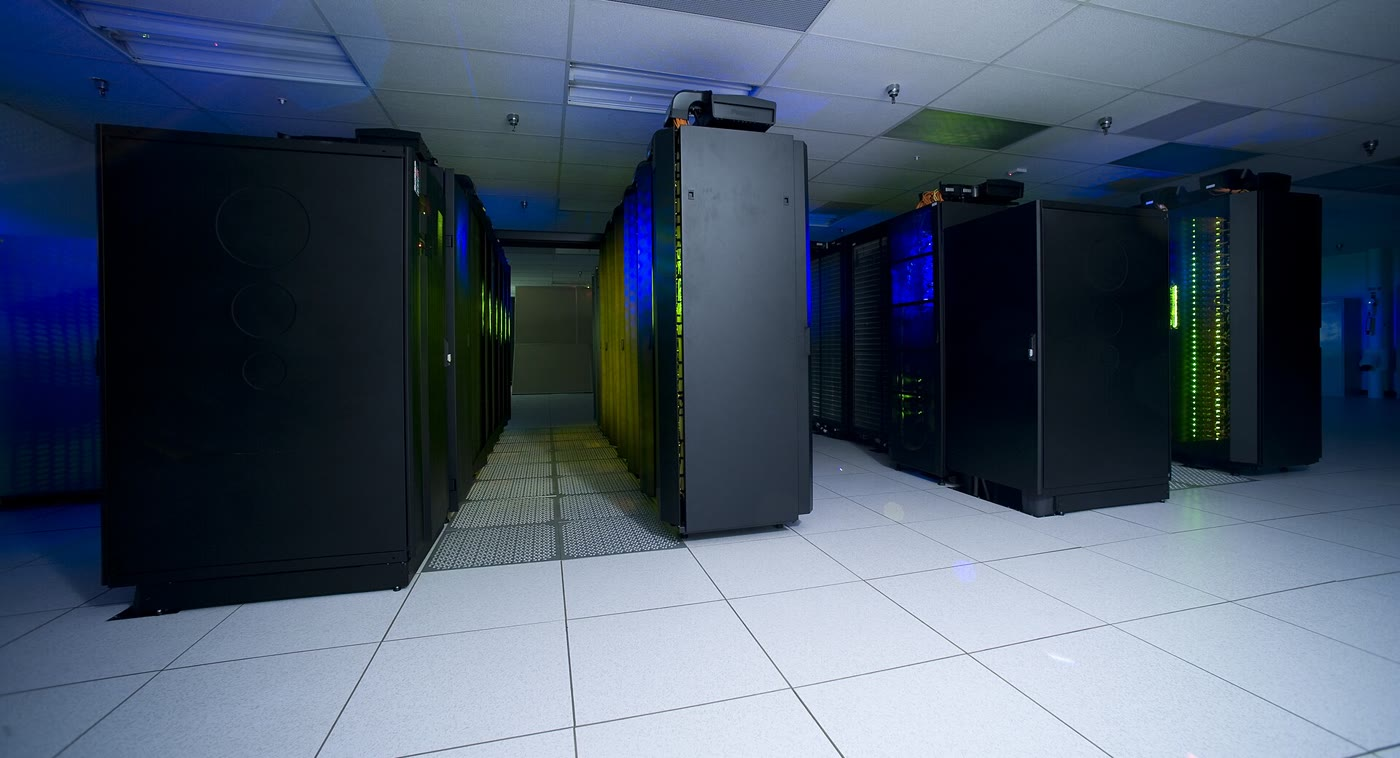
\includegraphics[width=0.7\linewidth]{images/book5/b3-nccs-supercomputer.jpg}

\par\smallskip{\small सुपरकंप्यूटर के रैक, NASA Center for Climate Simulation,
Goddard Space Flight Center में, \num{2010} में (NASA,
सार्वजनिक डोमेन)। किसी वैश्विक मॉडल के समीकरण ऐसे उच्च-निष्पादन कंप्यूटरों
पर संख्यात्मक रूप से हल किए जाते हैं।}\label{fig:b3:climate-models:supercomputer}
\end{omfigure}
% ledger: photo:b3-nccs, ar6ch1:esm

\section{मॉडलों का मूल्यांकन}\label{sec:b3:climate-models:evaluation}

किसी मॉडल की जाँच देखे गए जलवायु से की जाती है; कठिनाई यह है कि
उसे भी उसी के अनुसार समायोजित किया गया है। हर \omterm{def:b3:climate-models:gcm}{प्राचलीकरण} के ऐसे प्राचल होते हैं जिनकी
स्वीकार्य परास भौतिकी और प्रेक्षण से तय होती है, और जैसे-जैसे घटक जोड़े जाते हैं,
मॉडलकार उन्हें तब तक परिष्कृत करते हैं जब तक अनुकृत जलवायु कुछ ट्यूनिंग लक्ष्यों पर खरी न उतरे:
माध्य जलवायु --- उदाहरण के लिए, माध्य तापमान, जो
आज के सूर्यप्रकाश में प्रेक्षित तापमान के निकट हो --- क्षेत्रीय विशेषताएँ, या
ऐतिहासिक काल की प्रवृत्तियाँ। तभी मॉडल
अंतर-तुलनाओं के लिए जारी किया जाता है।
% ledger: ar6ch1:models, ar6ch1:parameterization, ar6ch1:large-ensembles

\begin{definition}[मॉडल अंतर-तुलना परियोजना]\label{def:b3:climate-models:cmip}
\emph{मॉडल अंतर-तुलना परियोजना}\index{मॉडल अंतर-तुलना परियोजना}
प्रयोगों का एक समन्वित समूह है --- वही बल, वही प्रोटोकॉल, वही निर्गम ---
जिसे कई मॉडलिंग समूह अपने-अपने मॉडलों से चलाते हैं, ताकि परिणामों की तुलना
की जा सके। युग्मित मॉडल अंतर-तुलना परियोजना (CMIP) क्रमिक चरणों में
चलती है; इसका छठा चरण,
CMIP6, छठे आकलन का एक प्रमुख साक्ष्य-स्रोत रहा।
\end{definition}

\begin{dated}{2021}
CMIP6 के जिन \num{29} मॉडलिंग समूहों ने बताया कि उन्होंने ट्यूनिंग कैसे की, उनमें से \num{23} ने
अपने मॉडल को ऐतिहासिक काल में प्रेक्षित तापन से ट्यून नहीं किया, और
\num{25} ने उसकी ECS को ट्यून नहीं किया: अधिकांश मॉडलों की संवेदनशीलता एक उद्भूत
गुण है, निवेश नहीं। औसतन CMIP6 मॉडलों की ECS और
TCR पिछले चरण के मॉडलों से अधिक हैं, और उनका प्रसार
रिपोर्ट द्वारा आकलन की गई परासों से चौड़ा है; कुछ मॉडलों में इसका कारण
मध्य और उच्च अक्षांशों के बादलों की प्रतिपुष्टि पाया गया। कुछ सबसे संवेदनशील मॉडल
हाल के प्रेक्षित तापन और अतीत की जलवायु को कम अच्छी तरह दोहराते हैं।
इसलिए आकलन ने ECS और TCR की परासें मॉडलों से सीधे नहीं लीं,
बल्कि प्रतिपुष्टि प्रक्रियाओं की समझ से,
उपकरणीय अभिलेख, अतीत की जलवायु और उद्भूत व्यवरोधों से लीं; वह सबसे संवेदनशील मॉडलों को
कम संभाविता और उच्च प्रभाव वाले परिणामों के मार्गदर्शक के रूप में लेता है (\emph{उच्च विश्वास})।
\end{dated}
% ledger: ar6ch1:models, ar6ch7:cmip6-sensitivity

\begin{definition}[बृहत् समष्टि; उद्भूत व्यवरोध]\label{def:b3:climate-models:evaluation}
\emph{बृहत् समष्टि}\index{बृहत् समष्टि} वह अनेक अनुकरणों का समूह है
जो एक ही मॉडल द्वारा, एक ही काल पर समान बलों के अंतर्गत किए जाते हैं,
और केवल अपनी आरंभिक अवस्थाओं में भिन्न होते हैं। \emph{उद्भूत
व्यवरोध}\index{उद्भूत व्यवरोध} वह संबंध है जो भिन्न-भिन्न मॉडलों की
एक समष्टि में पाया जाता है और वर्तमान जलवायु की किसी प्रेक्षणीय राशि
और भविष्य की किसी राशि, जैसे ECS, के बीच होता है; पहली का प्रेक्षित मान
फिर दूसरी की परास को संकीर्ण कर देता है।
\end{definition}

जलवायु अराजक है, इसलिए आरंभिक अवस्था के सूक्ष्म अंतर भी
\omterm{def:b3:climate-models:evaluation}{बृहत् समष्टि} के सदस्यों को भिन्न मार्गों पर भेज देते हैं: सदस्यों का प्रसार आंतरिक
परिवर्तनशीलता को मापता है, और उनका माध्य बाध्य
अनुक्रिया को। कई मॉडलों की बृहत् समष्टियों ने आकलन को समर्थन दिया। किसी \omterm{def:b3:climate-models:evaluation}{उद्भूत
व्यवरोध} को भौतिक कारण चाहिए। कुछ दर्जन मॉडलों में
हज़ारों प्रेक्षणीय राशियों को आज़माया जा सकता है, और कुछ संयोग से ECS से सहसंबद्ध निकल आएँगी;
आकलन ने उन्हें रखा जिनका भौतिक आधार था, जिनमें से कई
उष्णकटिबंधीय बादलों से संबंधित हैं, और चेतावनी दी कि
समष्टि के सभी मॉडलों में साझा पूर्वाग्रह इस विधि को निष्फल कर देता है।
% ledger: ar6ch1:large-ensembles, ar6ch7:emergent

\begin{inthelab}[एक मॉडलिंग केंद्र]
\begin{minipage}[t]{0.55\linewidth}\vspace{0pt}
एक जलवायु मॉडलिंग केंद्र में मॉडल एक ऐसा प्रोग्राम है जो एक दल द्वारा लिखा और
रखरखाव किया जाता है: वायुमंडल, महासागर, समुद्री हिम और भूमि अलग-अलग घटक हैं,
जो अपनी सीमाओं पर एक युग्मक के ज़रिए फ़्लक्स का आदान-प्रदान करते हैं। किसी चलाने से पहले
प्रयोग के बल पढ़े जाते हैं --- ग्रीनहाउस गैसों की सांद्रता,
एरोसोल, प्रोटोकॉल का भूमि उपयोग। ग्लोब को
टुकड़ों में बाँटा जाता है, जिन्हें सुपरकंप्यूटर के प्रोसेसर साथ-साथ गणना करते हैं,
और एक सदी की मॉडल जलवायु फ़ील्डों के एक बड़े
अभिलेख के रूप में लौटती है। वैज्ञानिक उन्हें स्क्रीनों पर दिखाते हैं,
पुनर्विश्लेषणों और उपग्रह अभिलेखों से उनकी तुलना करते हैं, और मानक निर्गम
अंतर-तुलना के अभिलेखागार को भेजते हैं, जहाँ अन्य समूह उनकी तुलना अपने मॉडलों से करते हैं।
\end{minipage}\hfill
\begin{minipage}[t]{0.42\linewidth}\vspace{0pt}
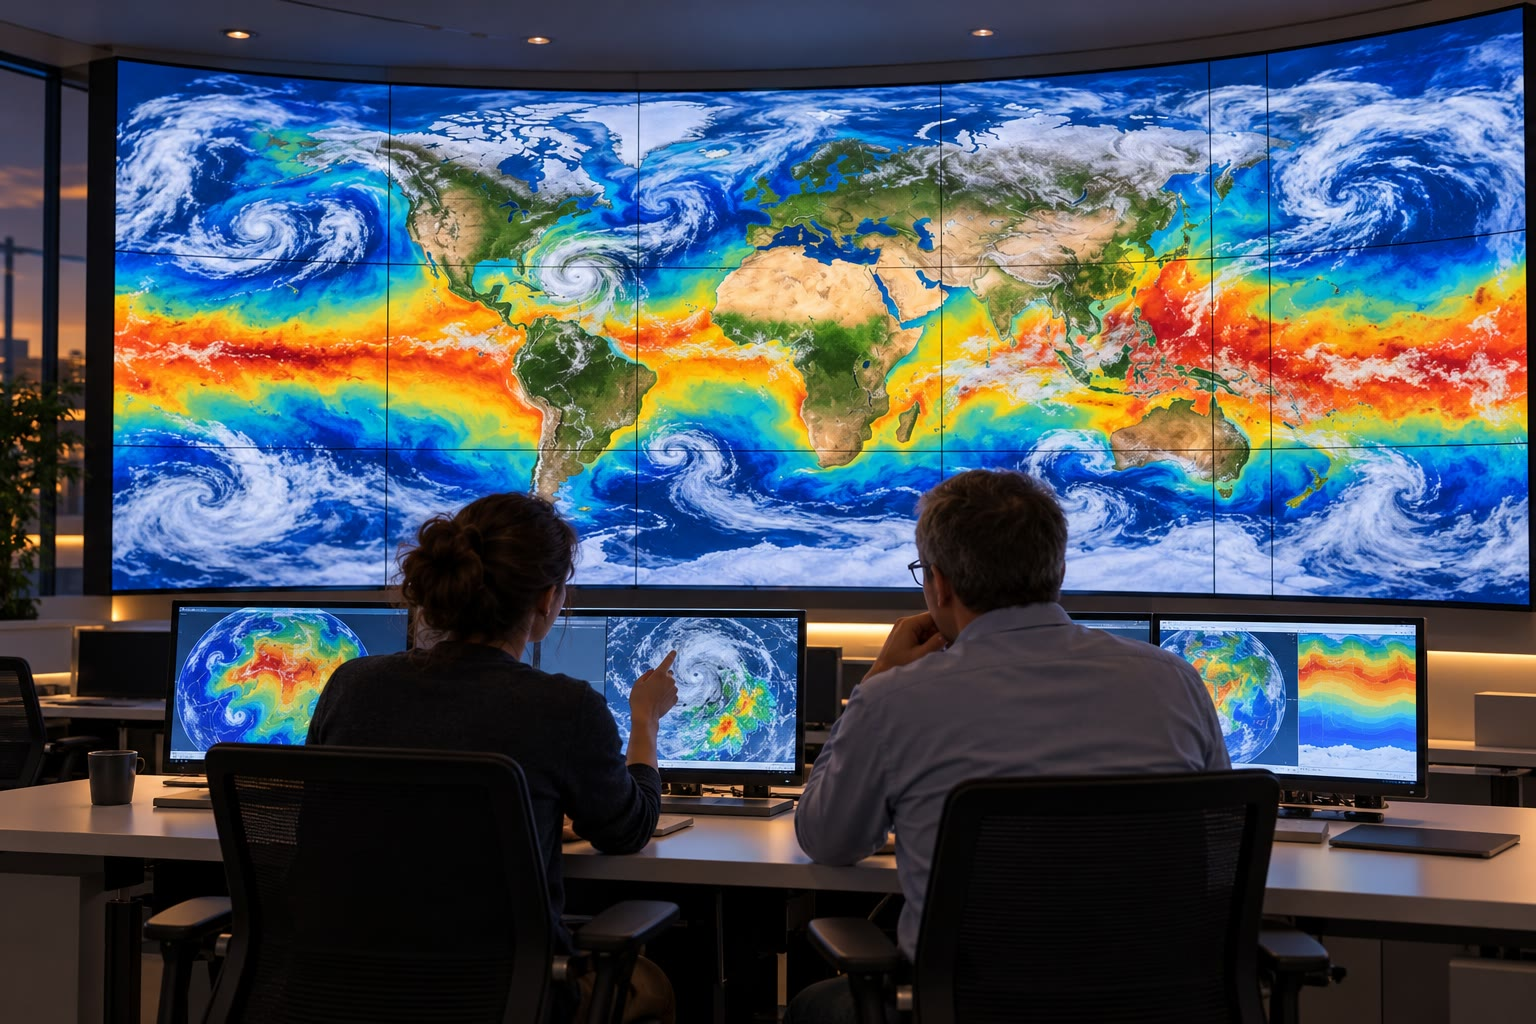
\includegraphics[width=\linewidth]{images/book5/ai/b3-model-centre.jpg}

{\scriptsize स्क्रीनों की एक दीवार के सामने दो वैज्ञानिक, जिन पर एक मॉडल चलने के
वैश्विक फ़ील्ड दिख रहे हैं (AI से बनाया गया चित्रण)।}
\end{minipage}
\end{inthelab}
% ledger: ar6ch1:esm, ar6ch1:models

\section{अभ्यास}

\begin{exercise}[$\star$]\label{exo:b3:climate-models:1}
बुडिको का OLR नियम है $I = a + bT - (a_1 + b_1T)n$, जहाँ $a = 14.0$, $b =
0.14$, $a_1 = 3.0$, $b_1 = 0.10$, \unit{kcal.cm^{-2}} प्रति माह में और $T$
\unit{\celsius} में। $n = 0.5$ के मेघाच्छादन के लिए $A$ और $B$ परिकलित कीजिए,
और उन्हें \unit{W/m^2} तथा \unit{W.m^{-2}.\celsius^{-1}} में बदलिए, जहाँ एक माह
365.25 दिनों वाले वर्ष का बारहवाँ भाग है। यह नियम
\qty{15}{\celsius} पर कितना OLR देता है?
\end{exercise}
% ledger: budyko69:olr

\begin{exercise}[$\star$]\label{exo:b3:climate-models:2}
$Q = \qty{340}{W/m^2}$, $A = \qty{211.9}{W/m^2}$ और $B =
\qty{1.816}{W.m^{-2}.\celsius^{-1}}$ के साथ साम्य तापमान परिकलित कीजिए,
एल्बिडो 0.30 और 0.31 के लिए। एल्बिडो में 0.01 की वृद्धि
इस ग्रह को कितना ठंडा करती है?
\end{exercise}

\begin{exercise}[$\star$]\label{exo:b3:climate-models:3}
समुद्री जल की मिश्रित परत, जिसकी गहराई
\qty{60}{m} है, उसकी प्रति वर्ग मीटर ऊष्माधारिता परिकलित कीजिए, जहाँ $\rho = \qty{1025}{kg/m^3}$ और $c_p = \qty{3992}{J.kg^{-1}.K^{-1}}$ है,
उसे \unit{J.m^{-2}.K^{-1}} और \unit{W.yr.m^{-2}.K^{-1}} में व्यक्त कीजिए।
\cref{thm:b3:climate-models:response} की अनुक्रिया-काल $\lambda = -B =
\qty{-1.816}{W.m^{-2}.\celsius^{-1}}$ और $\lambda =
\qty{-1.33}{W.m^{-2}.\celsius^{-1}}$ के लिए परिकलित कीजिए।
\end{exercise}
% ledger: teos10:cp0

\begin{exercise}[$\star$]\label{exo:b3:climate-models:4}
दो-परत मॉडल के लिए, जहाँ $\lambda = \qty{-1.33}{W.m^{-2}.\celsius^{-1}}$,
$\gamma = \qty{0.62}{W.m^{-2}.\celsius^{-1}}$ और $F_{2\times} =
\qty{3.93}{W/m^2}$ के साथ ECS, लगभग TCR $F_{2\times}/
(\gamma - \lambda)$, और इन दोनों का अनुपात परिकलित कीजिए।
\end{exercise}
% ledger: ar6sm7:two-layer, ipcc:erf-2xco2

\begin{exercise}[$\star\star$]\label{exo:b3:climate-models:5}
पाठ के शून्य-आयामी मॉडल में सौर स्थिरांक
\qty{1340}{W/m^2} लीजिए। तीनों साम्यावस्थाएँ ज्ञात कीजिए और प्रत्येक पर
शुद्ध फ़्लक्स की प्रवणता $N'(T)$ निकालिए; कौन-सी स्थायी हैं?
\end{exercise}

\begin{exercise}[$\star\star$]\label{exo:b3:climate-models:6}
पाठ के एल्बिडो रैंप को खिसकाइए: $\alpha = 0.62$ \qty{-20}{\celsius} से नीचे,
$0.30$ \qty{0}{\celsius} से ऊपर, बीच में रैखिक। $A$ और $B$ यथावत् रखिए। किस
सौर स्थिरांक पर उष्ण शाखा समाप्त होती है, और वह
\qty{1360}{W/m^2} से कितने प्रतिशत नीचे है? किस सौर स्थिरांक पर हिमगोल पिघलता है?
सीमा का आकार क्या तय करता है?
\end{exercise}

\begin{exercise}[$\star\star$]\label{exo:b3:climate-models:7}
पाठ के मापदंडों वाला एक मॉडल ग्रह हिमगोल अवस्था में है।
(क)~आज के सौर स्थिरांक पर इसका तापमान क्या है? (ख)~सूर्य को यथावत् रखते हुए,
कौन-सा प्रणोदन $F$ हिमगोल के तापमान को
\qty{-10}{\celsius} तक ले जाएगा? यह कार्बन डाइऑक्साइड के दोगुने होने के प्रणोदन
\qty{3.93}{W/m^2} का कितना गुना है? (ग)~बर्फ़ हट जाने के बाद, यदि प्रणोदन हटा दिया
जाए, तो ग्रह किस अवस्था में स्थिर होगा?
\end{exercise}
% ledger: ipcc:erf-2xco2, hoffman17:hysteresis

\begin{exercise}[$\star\star$]\label{exo:b3:climate-models:8}
मॉडल X, एक काल्पनिक दो-परत मॉडल, में $C = 7.0$ और $C_d =
\qty{90}{W.yr.m^{-2}.\celsius^{-1}}$, $\gamma = 0.70$ और $\lambda =
\qty{-1.10}{W.m^{-2}.\celsius^{-1}}$ है। इसके दोनों समय-मापक्रम ठीक-ठीक
तथा \cref{thm:b3:climate-models:two-layer} के सन्निकटनों से परिकलित कीजिए, साथ ही
अंश $a_f$, इसका ECS और लगभग TCR निकालिए।
\end{exercise}

\begin{exercise}[$\star\star$]\label{exo:b3:climate-models:9}
पाठ के बुडिको मॉडल में $\bar T = \qty{12.81}{\celsius}$, $\beta =
\qty{3.74}{W.m^{-2}.\celsius^{-1}}$, \ang{72} पर हिम-रेखा, विषुवत रेखा पर $s = 1.221$
और ध्रुव पर $0.506$, तथा $\alpha = 0.30$ और $0.62$ है।
विषुवत रेखा और ध्रुव पर तापमान परिकलित कीजिए, और
परिवहन द्वारा वहाँ से हटाई या वहाँ लाई गई ऊष्मा $\beta(T - \bar T)$
प्रति वर्ग मीटर निकालिए।
\end{exercise}

\begin{exercise}[$\star\star\star$]\label{exo:b3:climate-models:10}
बिना हिम वाले एक ग्रह ($\alpha = 0.30$ सर्वत्र) में विसरणी परिवहन
$D = -\mathcal D\,\partial_x[(1 - x^2)\partial_xT]$ तथा सूर्यातप
$s(x) = 1 + s_2P_2(x)$, $P_2 = (3x^2 - 1)/2$ है। (क)~दिखाइए कि
$\partial_x[(1 - x^2)\partial_xP_2] = -6P_2$। (ख)~दिखाइए कि $T = T_0 +
T_2P_2(x)$ एक स्थायी हल है, जहाँ $T_0 = (Q(1 - \alpha) - A)/B$ और
$T_2 = Qs_2(1 - \alpha)/(B + 6\mathcal D)$ है। (ग)~पुनर्विश्लेषण का सूर्यातप
$s_2 = \num{-0.476}$ देता है। परिवहन के बिना विषुवत रेखा और ध्रुव के बीच
तापमान का अंतर क्या होगा? (घ)~कौन-सा $\mathcal D$ प्रेक्षित
अंतर, \qty{55.3}{\celsius}, देता है?
\end{exercise}
% ledger: data:b3-ncep, data:b5-ncep-air

\begin{exercise}[$\star\star\star$]\label{exo:b3:climate-models:11}
(क)~\cref{thm:b3:climate-models:two-layer} के द्विघात समीकरण को $r^2 -
\Sigma r + \Pi = 0$ के रूप में लिखिए और दिखाइए कि यदि $4\Pi \ll \Sigma^2$ हो, तो इसके मूल
$\Sigma$ और $\Pi/\Sigma$ के लगभग बराबर होते हैं। (ख)~एक रैखिक रूप से बढ़ते प्रणोदन $F = kt$ के लिए
दिखाइए कि जब $t \gg \tau_f$ हो, और जब तक $T_d$ छोटा रहता है,
$T \approx kt/(\gamma - \lambda)$ होता है; इससे लगभग TCR निकालिए। (ग)~
पाठ की संख्याएँ जाँचिए: $\Sigma$, $\Pi$, दोनों समय-मापक्रम, और
अनुपात $4\Pi/\Sigma^2$।
\end{exercise}
% ledger: ar6sm7:two-layer

\begin{exercise}[$\star\star\star$]\label{exo:b3:climate-models:12}
एक काल्पनिक आठ मॉडलों की समष्टि वर्तमान जलवायु का एक प्रेक्षणीय $X$ और
उनका ECS देती है:
\begin{center}
\begin{tabular}{l*{8}{c}}
\hline
$X$ & 0.2 & 0.5 & 0.6 & 0.8 & 1.0 & 1.1 & 1.3 & 1.5\\
ECS (\unit{\celsius}) & 2.3 & 2.7 & 3.1 & 3.2 & 3.8 & 3.9 & 4.4 & 4.6\\
\hline
\end{tabular}
\end{center}
(क)~समष्टि के ECS का माध्य और मानक विचलन परिकलित कीजिए।
(ख)~न्यूनतम वर्ग से ECS $= a + bX$ का समंजन कीजिए; सहसंबंध
और अवशिष्टों का मानक विचलन परिकलित कीजिए। (ग)~प्रेक्षित $X$ $0.7
\pm 0.1$ है। यह व्यवरोध कौन-सा ECS देता है, और किस प्रसार के साथ?
(घ)~किस बात से आप इस व्यवरोध पर संदेह करेंगे?
\end{exercise}
% ledger: ar6ch7:emergent

\section{समस्या: हिमगोल से कितना निकट?}

\begin{problem}[{सप्ताहांत समस्या --- साम्यावस्थाएँ, स्थायित्व और
हिमाच्छादन देहली}]
\label{pb:b3:climate-models:1}
एक मॉडल ग्रह का आज का सौर स्थिरांक $S_0 = \qty{1360}{W/m^2}$ है और
OLR नियम $A + BT$ है, जहाँ $A = \qty{211.9}{W/m^2}$ और $B =
\qty{1.816}{W.m^{-2}.\celsius^{-1}}$ है। इसका एल्बिडो
\qty{-10}{\celsius} से नीचे 0.62, \qty{+10}{\celsius} से ऊपर 0.30, बीच में रैखिक, और
इसकी पृष्ठ ऊष्मा धारिता $C = \qty{8.1}{W.yr.m^{-2}.\celsius^{-1}}$ है।
$\sigma = \qty{5.670e-8}{W.m^{-2}.K^{-4}}$ मान लीजिए।

\medskip\noindent\textbf{भाग I --- संतुलन में ग्रह।}
\begin{enumerate}
\item ग्रह के प्रति वर्ग मीटर औसत सूर्यप्रकाश $Q_0$ परिकलित कीजिए, और
  इस गुणक को समझाइए।
\item एल्बिडो 0.30 के साथ अवशोषित सूर्यप्रकाश और
  \qty{15}{\celsius} पर OLR परिकलित कीजिए।
\item उष्ण साम्यावस्था परिकलित कीजिए।
\item हिमगोल साम्यावस्था परिकलित कीजिए, और जाँच कीजिए कि वह
  हिम शाखा पर स्थित है।
\item एल्बिडो रैंप पर स्थित तीसरी साम्यावस्था परिकलित कीजिए।
\item अवशोषित सूर्यप्रकाश को कृष्ण पिंड के रूप में अंतरिक्ष में
  वापस भेजने वाला उत्सर्जन तापमान परिकलित कीजिए, और उसकी उष्ण साम्यावस्था से तुलना कीजिए।
\end{enumerate}

\medskip\noindent\textbf{भाग II --- स्थायित्व और समय।}
\begin{enumerate}[resume]
\item प्रत्येक साम्यावस्था पर शुद्ध फ़्लक्स की प्रवणता $N'(T)$ परिकलित कीजिए, और बताइए
  कौन-कौन स्थायी हैं।
\item मध्यवर्ती साम्यावस्था से एक छोटा विचलन $\mathrm
  e^{t/\tau}$ के रूप में बढ़ता है। $\tau$ परिकलित कीजिए।
\item उष्ण साम्यावस्था का अनुक्रिया काल परिकलित कीजिए।
\item \qty{3.93}{W/m^2} का विकिरणी प्रणोदन, जो कार्बन डाइऑक्साइड के दोगुने
  होने के बराबर है, चालू कर दिया जाता है। साम्य पर तापन परिकलित कीजिए, और
  उसकी तुलना वास्तविक जलवायु के लिए आकलित ECS से कीजिए।
\item मॉडल को तापन का \qty{95}{\percent} पूरा करने में
  कितना समय लगता है? वास्तविक जलवायु को अधिक समय क्यों लगता है?
\end{enumerate}

\medskip\noindent\textbf{भाग III --- सैडल-नोड द्विभाजन।}
\begin{enumerate}[resume]
\item जैसे-जैसे सूर्य मंद होता है, किस तापमान पर उष्ण साम्यावस्था
  मध्यवर्ती साम्यावस्था से मिलती है? वहाँ $Q$ परिकलित कीजिए।
\item द्विभाजन पर सौर स्थिरांक, और आज से उसकी प्रतिशत में
  गिरावट परिकलित कीजिए।
\item उसके ठीक नीचे जलवायु कहाँ जाती है? उसका तापमान परिकलित कीजिए।
\item जिस सौर स्थिरांक पर हिमगोल गलता है, उसे परिकलित कीजिए, और
  आज से उसकी प्रतिशत में वृद्धि भी दीजिए।
\item जब $S_0$ को घटाकर द्विभाजन से नीचे ले जाया जाता है और
  \qty{1360}{W/m^2} पर वापस लाया जाता है, तब तापमान द्वारा अनुसरित पाश का रेखाचित्र बनाइए।
\end{enumerate}

\medskip\noindent\textbf{भाग IV --- हिम रेखा।} ग्रह के लिए
बुडिको का अक्षांशीय मॉडल, जिसमें $\beta = \qty{3.739}{W.m^{-2}.\celsius^{-1}}$ है, और
हिम एल्बिडो हिम रेखा के ध्रुव की ओर 0.62, भूमध्य की ओर 0.30, किनारे पर 0.50
और पुनर्विश्लेषण का सूर्यातप लेकर अपनाइए:
\begin{center}
\begin{tabular}{lccccccc}
\hline
अक्षांश & \ang{0} & \ang{30} & \ang{40} & \ang{47.5} & \ang{55} & \ang{60} & \ang{72}\\
$s(x_s)$ & 1.2211 & 1.0730 & 0.9647 & 0.8688 & 0.7650 & 0.6947 & 0.5643\\
$F(x_s)$ & 0 & 0.5865 & 0.7324 & 0.8192 & 0.8863 & 0.9205 & 0.9738\\
\hline
\end{tabular}
\end{center}
\begin{enumerate}[resume]
\item हिम रेखा \ang{72} पर होने पर माध्य एल्बिडो $\bar\alpha$
  और माध्य तापमान $\bar T$ परिकलित कीजिए।
\item वह क्रांतिक तापमान $T_c$ परिकलित कीजिए, जिस पर किनारा
  आज \ang{72} पर होता है, और पुनर्विश्लेषण के मान \qty{-15.8}{\celsius} से उसकी तुलना कीजिए।
\item \cref{prop:b3:climate-models:iceline} में $Q(x_s)$ का अंश
  और अनुपात $\beta/B$ परिकलित कीजिए।
\item हिम रेखा \ang{30}, \ang{40},
  \ang{47.5}, \ang{55} और \ang{60} के लिए $Q(x_s)/Q_0$ परिकलित कीजिए।
\item इन मानों का न्यूनतम कहाँ है? कौन-सी हिम रेखाएँ स्थायी हैं?
\item आज के सूर्य के साथ मॉडल कौन-सी अन्य हिम रेखा की अनुमति देता है, और क्या वह
  स्थायी है? क्या आज हिमगोल संभव है? (स्तंभ \ang{0} का उपयोग कीजिए।)
\item अक्षांशीय मॉडल की देहली की तुलना भाग~III की देहली से,
  बुडिको के \qty{1.6}{\percent} से, और देहली पर हिम के अक्षांश की
  उनके \ang{50} से तुलना कीजिए।
\item मॉडल ग्रह को जो हिमाच्छादित कर देती है, सौर स्थिरांक की उस गिरावट को
  दो सार्थक अंकों तक, प्रतिशत में दीजिए।
\end{enumerate}
\end{problem}
% ledger: nasa:solar-mean, data:b5-ncep-air, data:b3-ncep, budyko69:transport, budyko69:albedo, budyko69:threshold, ipcc:ecs, const:sigma
